\section{Algorithm performance}
\label{sec:perf}

\renewcommand{\arraystretch}{1.2} % maybe 1.3?
\begin{table*}[!htb]
  \centering
  \caption{%
    Results of timing the Hypersliceplorer algorithm on a number of different
    datasets. I ran the algorithm setting the number of slices to $1,000$.
    I record the number of simplices created by the quickhull
    algorithm~\cite{Barber:1996}, the total time for all slices, and the time
    per simplex. The time per simplex is the total time divided by the number
    of plots (i.e.\ dimension pairs, the number of simplices, and the number of focus points.
    The time per simplex is roughly constant.
  } 
  \label{tbl:timings}
  \begin{tabular}[]{@{}lcrrr@{}} \toprule
    Dataset & Dims & Simplices & Total time (sec) & Time/simplex (ms) \\
    \midrule
    %\endhead
    Cube & 3 & 12 & 48 & 1.345 \\
    Octahedron & 3 & 8 & 38 & 1.624 \\
    Sphere & 3 & 596 & 1,243 & 0.696 \\
    Tesseract & 4 & 58 & 289 & 0.833 \\
    16-cell & 4 & 16 & 108 & 1.135 \\
    3-sphere & 4 & 2,567 & 14,283 & 0.927 \\
    5d-cube & 5 & 316 & 2,378 & 0.753 \\
    5d-ortho & 5 & 32 & 258 & 0.808 \\
    4-sphere & 5 & 12,886 & 130,453 & 1.012 \\
    Klein bottle & 4 & 36,258 & 129,158 & 0.594 \\
    \bottomrule
  \end{tabular}
\end{table*}

\begin{figure}
  \centering
  \resizebox{\linewidth}{0.7\linewidth}{%
    % Created by tikzDevice version 0.10.1 on 2017-12-13 11:15:52
% !TEX encoding = UTF-8 Unicode
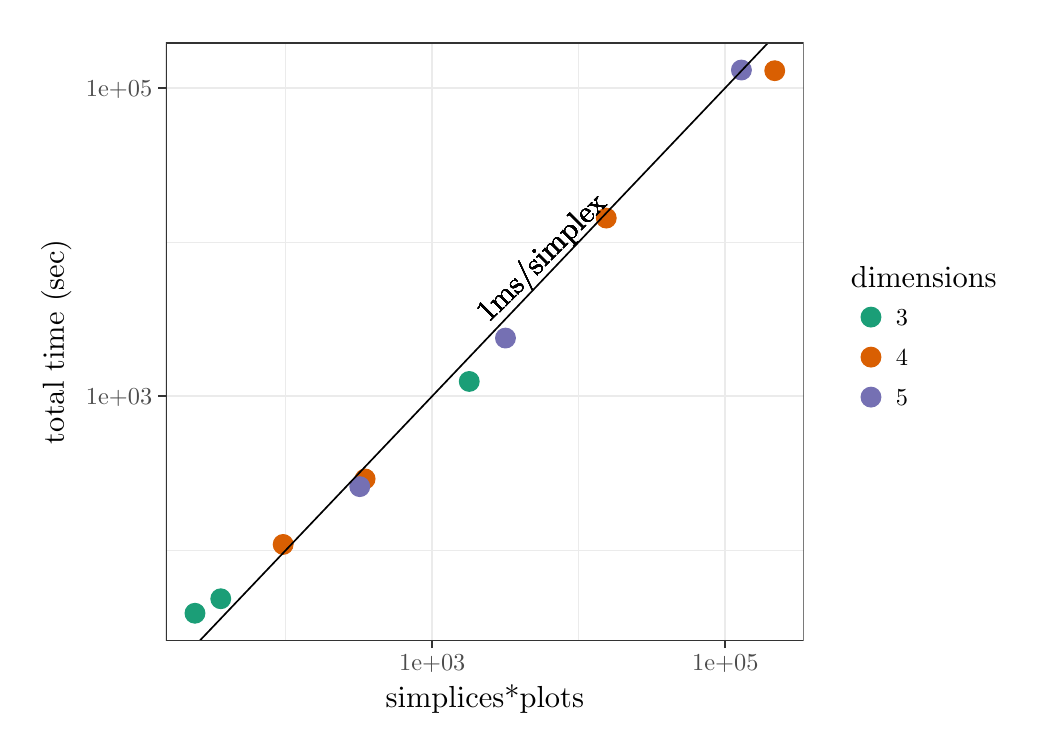
\begin{tikzpicture}[x=1pt,y=1pt]
\definecolor{fillColor}{RGB}{255,255,255}
\path[use as bounding box,fill=fillColor,fill opacity=0.00] (0,0) rectangle (361.35,252.94);
\begin{scope}
\path[clip] (  0.00,  0.00) rectangle (361.35,252.94);
\definecolor{drawColor}{RGB}{255,255,255}
\definecolor{fillColor}{RGB}{255,255,255}

\path[draw=drawColor,line width= 0.6pt,line join=round,line cap=round,fill=fillColor] (  0.00, -0.00) rectangle (361.35,252.94);
\end{scope}
\begin{scope}
\path[clip] ( 49.98, 31.53) rectangle (280.42,247.45);
\definecolor{fillColor}{RGB}{255,255,255}

\path[fill=fillColor] ( 49.98, 31.53) rectangle (280.42,247.45);
\definecolor{drawColor}{gray}{0.92}

\path[draw=drawColor,line width= 0.3pt,line join=round] ( 49.98, 64.13) --
	(280.42, 64.13);

\path[draw=drawColor,line width= 0.3pt,line join=round] ( 49.98,175.51) --
	(280.42,175.51);

\path[draw=drawColor,line width= 0.3pt,line join=round] ( 93.26, 31.53) --
	( 93.26,247.45);

\path[draw=drawColor,line width= 0.3pt,line join=round] (199.14, 31.53) --
	(199.14,247.45);

\path[draw=drawColor,line width= 0.6pt,line join=round] ( 49.98,119.82) --
	(280.42,119.82);

\path[draw=drawColor,line width= 0.6pt,line join=round] ( 49.98,231.20) --
	(280.42,231.20);

\path[draw=drawColor,line width= 0.6pt,line join=round] (146.20, 31.53) --
	(146.20,247.45);

\path[draw=drawColor,line width= 0.6pt,line join=round] (252.08, 31.53) --
	(252.08,247.45);
\definecolor{drawColor}{RGB}{27,158,119}
\definecolor{fillColor}{RGB}{27,158,119}

\path[draw=drawColor,line width= 0.4pt,line join=round,line cap=round,fill=fillColor] ( 69.77, 46.58) circle (  3.57);

\path[draw=drawColor,line width= 0.4pt,line join=round,line cap=round,fill=fillColor] ( 60.45, 41.34) circle (  3.57);
\definecolor{drawColor}{RGB}{217,95,2}
\definecolor{fillColor}{RGB}{217,95,2}

\path[draw=drawColor,line width= 0.4pt,line join=round,line cap=round,fill=fillColor] (121.93, 89.87) circle (  3.57);

\path[draw=drawColor,line width= 0.4pt,line join=round,line cap=round,fill=fillColor] ( 92.32, 66.20) circle (  3.57);
\definecolor{drawColor}{RGB}{117,112,179}
\definecolor{fillColor}{RGB}{117,112,179}

\path[draw=drawColor,line width= 0.4pt,line join=round,line cap=round,fill=fillColor] (172.65,140.78) circle (  3.57);

\path[draw=drawColor,line width= 0.4pt,line join=round,line cap=round,fill=fillColor] (120.00, 87.10) circle (  3.57);
\definecolor{drawColor}{RGB}{217,95,2}
\definecolor{fillColor}{RGB}{217,95,2}

\path[draw=drawColor,line width= 0.4pt,line join=round,line cap=round,fill=fillColor] (269.95,237.39) circle (  3.57);
\definecolor{drawColor}{RGB}{27,158,119}
\definecolor{fillColor}{RGB}{27,158,119}

\path[draw=drawColor,line width= 0.4pt,line join=round,line cap=round,fill=fillColor] (159.56,125.10) circle (  3.57);
\definecolor{drawColor}{RGB}{217,95,2}
\definecolor{fillColor}{RGB}{217,95,2}

\path[draw=drawColor,line width= 0.4pt,line join=round,line cap=round,fill=fillColor] (209.07,184.13) circle (  3.57);
\definecolor{drawColor}{RGB}{117,112,179}
\definecolor{fillColor}{RGB}{117,112,179}

\path[draw=drawColor,line width= 0.4pt,line join=round,line cap=round,fill=fillColor] (257.91,237.63) circle (  3.57);
\definecolor{drawColor}{RGB}{0,0,0}

\path[draw=drawColor,line width= 0.6pt,line join=round] ( 49.98, 18.59) -- (272.75,252.94);

\node[text=drawColor,rotate= 45.00,anchor=base,inner sep=0pt, outer sep=0pt, scale=  1.10] at (188.08,167.42) {1ms/simplex};

\node[text=drawColor,rotate= 45.00,anchor=base,inner sep=0pt, outer sep=0pt, scale=  1.10] at (188.08,167.42) {1ms/simplex};

\node[text=drawColor,rotate= 45.00,anchor=base,inner sep=0pt, outer sep=0pt, scale=  1.10] at (188.08,167.42) {1ms/simplex};

\node[text=drawColor,rotate= 45.00,anchor=base,inner sep=0pt, outer sep=0pt, scale=  1.10] at (188.08,167.42) {1ms/simplex};

\node[text=drawColor,rotate= 45.00,anchor=base,inner sep=0pt, outer sep=0pt, scale=  1.10] at (188.08,167.42) {1ms/simplex};

\node[text=drawColor,rotate= 45.00,anchor=base,inner sep=0pt, outer sep=0pt, scale=  1.10] at (188.08,167.42) {1ms/simplex};

\node[text=drawColor,rotate= 45.00,anchor=base,inner sep=0pt, outer sep=0pt, scale=  1.10] at (188.08,167.42) {1ms/simplex};

\node[text=drawColor,rotate= 45.00,anchor=base,inner sep=0pt, outer sep=0pt, scale=  1.10] at (188.08,167.42) {1ms/simplex};

\node[text=drawColor,rotate= 45.00,anchor=base,inner sep=0pt, outer sep=0pt, scale=  1.10] at (188.08,167.42) {1ms/simplex};

\node[text=drawColor,rotate= 45.00,anchor=base,inner sep=0pt, outer sep=0pt, scale=  1.10] at (188.08,167.42) {1ms/simplex};
\definecolor{drawColor}{gray}{0.20}

\path[draw=drawColor,line width= 0.6pt,line join=round,line cap=round] ( 49.98, 31.53) rectangle (280.42,247.45);
\end{scope}
\begin{scope}
\path[clip] (  0.00,  0.00) rectangle (361.35,252.94);
\definecolor{drawColor}{gray}{0.30}

\node[text=drawColor,anchor=base east,inner sep=0pt, outer sep=0pt, scale=  0.88] at ( 45.03,116.79) {1e+03};

\node[text=drawColor,anchor=base east,inner sep=0pt, outer sep=0pt, scale=  0.88] at ( 45.03,228.17) {1e+05};
\end{scope}
\begin{scope}
\path[clip] (  0.00,  0.00) rectangle (361.35,252.94);
\definecolor{drawColor}{gray}{0.20}

\path[draw=drawColor,line width= 0.6pt,line join=round] ( 47.23,119.82) --
	( 49.98,119.82);

\path[draw=drawColor,line width= 0.6pt,line join=round] ( 47.23,231.20) --
	( 49.98,231.20);
\end{scope}
\begin{scope}
\path[clip] (  0.00,  0.00) rectangle (361.35,252.94);
\definecolor{drawColor}{gray}{0.20}

\path[draw=drawColor,line width= 0.6pt,line join=round] (146.20, 28.78) --
	(146.20, 31.53);

\path[draw=drawColor,line width= 0.6pt,line join=round] (252.08, 28.78) --
	(252.08, 31.53);
\end{scope}
\begin{scope}
\path[clip] (  0.00,  0.00) rectangle (361.35,252.94);
\definecolor{drawColor}{gray}{0.30}

\node[text=drawColor,anchor=base,inner sep=0pt, outer sep=0pt, scale=  0.88] at (146.20, 20.52) {1e+03};

\node[text=drawColor,anchor=base,inner sep=0pt, outer sep=0pt, scale=  0.88] at (252.08, 20.52) {1e+05};
\end{scope}
\begin{scope}
\path[clip] (  0.00,  0.00) rectangle (361.35,252.94);
\definecolor{drawColor}{RGB}{0,0,0}

\node[text=drawColor,anchor=base,inner sep=0pt, outer sep=0pt, scale=  1.10] at (165.20,  7.44) {simplices*plots};
\end{scope}
\begin{scope}
\path[clip] (  0.00,  0.00) rectangle (361.35,252.94);
\definecolor{drawColor}{RGB}{0,0,0}

\node[text=drawColor,rotate= 90.00,anchor=base,inner sep=0pt, outer sep=0pt, scale=  1.10] at ( 13.08,139.49) {total time (sec)};
\end{scope}
\begin{scope}
\path[clip] (  0.00,  0.00) rectangle (361.35,252.94);
\definecolor{fillColor}{RGB}{255,255,255}

\path[fill=fillColor] (291.80,106.52) rectangle (355.85,172.45);
\end{scope}
\begin{scope}
\path[clip] (  0.00,  0.00) rectangle (361.35,252.94);
\definecolor{drawColor}{RGB}{0,0,0}

\node[text=drawColor,anchor=base west,inner sep=0pt, outer sep=0pt, scale=  1.10] at (297.49,159.19) {dimensions};
\end{scope}
\begin{scope}
\path[clip] (  0.00,  0.00) rectangle (361.35,252.94);
\definecolor{fillColor}{RGB}{255,255,255}

\path[fill=fillColor] (297.49,141.12) rectangle (311.95,155.57);
\end{scope}
\begin{scope}
\path[clip] (  0.00,  0.00) rectangle (361.35,252.94);
\definecolor{drawColor}{RGB}{27,158,119}
\definecolor{fillColor}{RGB}{27,158,119}

\path[draw=drawColor,line width= 0.4pt,line join=round,line cap=round,fill=fillColor] (304.72,148.35) circle (  3.57);
\end{scope}
\begin{scope}
\path[clip] (  0.00,  0.00) rectangle (361.35,252.94);
\definecolor{fillColor}{RGB}{255,255,255}

\path[fill=fillColor] (297.49,126.67) rectangle (311.95,141.12);
\end{scope}
\begin{scope}
\path[clip] (  0.00,  0.00) rectangle (361.35,252.94);
\definecolor{drawColor}{RGB}{217,95,2}
\definecolor{fillColor}{RGB}{217,95,2}

\path[draw=drawColor,line width= 0.4pt,line join=round,line cap=round,fill=fillColor] (304.72,133.89) circle (  3.57);
\end{scope}
\begin{scope}
\path[clip] (  0.00,  0.00) rectangle (361.35,252.94);
\definecolor{fillColor}{RGB}{255,255,255}

\path[fill=fillColor] (297.49,112.21) rectangle (311.95,126.67);
\end{scope}
\begin{scope}
\path[clip] (  0.00,  0.00) rectangle (361.35,252.94);
\definecolor{drawColor}{RGB}{117,112,179}
\definecolor{fillColor}{RGB}{117,112,179}

\path[draw=drawColor,line width= 0.4pt,line join=round,line cap=round,fill=fillColor] (304.72,119.44) circle (  3.57);
\end{scope}
\begin{scope}
\path[clip] (  0.00,  0.00) rectangle (361.35,252.94);
\definecolor{drawColor}{RGB}{0,0,0}

\node[text=drawColor,anchor=base west,inner sep=0pt, outer sep=0pt, scale=  0.88] at (313.75,145.32) {3};
\end{scope}
\begin{scope}
\path[clip] (  0.00,  0.00) rectangle (361.35,252.94);
\definecolor{drawColor}{RGB}{0,0,0}

\node[text=drawColor,anchor=base west,inner sep=0pt, outer sep=0pt, scale=  0.88] at (313.75,130.86) {4};
\end{scope}
\begin{scope}
\path[clip] (  0.00,  0.00) rectangle (361.35,252.94);
\definecolor{drawColor}{RGB}{0,0,0}

\node[text=drawColor,anchor=base west,inner sep=0pt, outer sep=0pt, scale=  0.88] at (313.75,116.41) {5};
\end{scope}
\end{tikzpicture}

  }
  \caption{%
    Chart showing the number of slicing operations 
    (simplices $\times$ number of plots) versus timing results from running 
    our algorithm on a number of different datasets. The axes are on a log-log
    scale. The points are all clustered around the ``1 ms/simplex'' line 
    showing that the running time is roughly one millisecond per slicing 
    operation.
  }
  \label{fig:timing}
\end{figure}

In order to test the running time of the slicing algorithm I ran a number of
experiments to understand the timing. I tested regular polytopes in 3, 4, and
5 dimensions as well as hyperspheres. I also tested the four-dimensional
version of the Klein bottle because it has a large number of simplices in its
mesh. For each test, I ran the slicing algorithm for all pairs of dimensions
and for $1,000$ focus points. I recorded the total wall clock time as well as
the number of simplices given by the quickhull algorithm. The testing machine
has an 8-core 3.2GHz Intel i7-6900K with 64GB of RAM.

The results are shown in \autoref{tbl:timings}. The total number of slicing
checks (\autoref{alg:slicing:single}) is the number of simplices, times the
number of pairs of dimensions ($d \choose 2$), times the total number of focus
points ($1,000$). I divide the total time by this number to show the time per
simplex. 

As we can see, the times are roughly constant between the number of
dimensions and simplices (see \autoref{fig:timing}). The reason the Klein 
bottle is faster is because
many slices do not hit any simplices and the algorithm will exit early
once this is detected. Right now this algorithm is not optimized.
For example, it would be greatly beneficial to pre-compute a spatial data
structure so that only slices that are likely to intersect simplices are
evaluated. Currently, the algorithm must check every simplex against every
focus point for every pair of dimensions. This is a lot of extra work for figures
such as the Klein bottle with many simplexes.

